\documentclass[addpoints,12pt]{exam}
%\documentclass[14pt]{exam}
\newcommand{\ds}{\displaystyle}
\usepackage[margin=0.8in]{geometry}
\usepackage{subcaption}
\usepackage{tikz}
\usepackage{amssymb,amsmath,graphicx,wrapfig,verbatim, psfragx,color}
\usepackage{multicol}
\usepackage{wasysym}
\def\FillInBlank{\rule{3truein} {.01truein}}
% Choose one option (bubbles)
\newcommand{\chooseone}{{\Large$\Circle$\ \ }}
\usepackage{amssymb,amsmath,graphicx,wrapfig,verbatim, psfragx,color}
\usepackage{multicol}
% If you want them as a list (instead of next to each other)
\usepackage{enumitem}
% ---- Convenience commands -----
% Choose one option (bubbles)
%\newcommand{\chooseone}{{\Large$\Circle$\ \ }}
% ---- Example Usage | Multiple Choice -----
%\usepackage{fancyhdr}
%\setlength{\headheight}{13.6pt}
%\pagestyle{fancy}
%\lhead{Math 222}
%\chead{ Midterm 1 }
%\rhead{Spring 2022}
\def\FillInBlank{\rule{3truein} {.01truein}}
\newcommand{\TorF}{\hspace{.1in} \textbf{True} \hspace{.1in} \textbf{False} \hspace{.1in}}
\begin{document}
\begin{enumerate}
\item Let $\vec{a} = \langle 2, -3, 1 \rangle $ and $\vec{b} = \langle 1, 4, -2 \rangle.$
\begin{itemize}
\item[3] Find the unit vector in the direction of $\vec{a}.$
\vfill
%\item Find the area of the parallelogram spanned by the vectors $\vec{a}$ and $\vec{b}.$
%\vfill
\item[5] Find the vector projection of $\vec{b}$ onto $\vec{a}.$
\vfill
\end{itemize}
\newpage
\item[8] Find an equation for the plane that contains the points $A = (1,0,1),$ $B = (3, 2, 0)$
and $C = (4, 1, 2).$
\newpage
\item[6] Find an equation for the {\bf line segment} connecting the points $A = (1,4, 2)$ and
$B = (5, 3, 8).$
\newpage
\item Consider the surface $x^2 =4y^2 + z^2$.
\begin{itemize}
\item[3] Sketch the traces of the form $x = k$, with $ k =0, 1$ in the $yz$-plane where the $y$
axis is horizontal. Label your traces.
\begin{center}
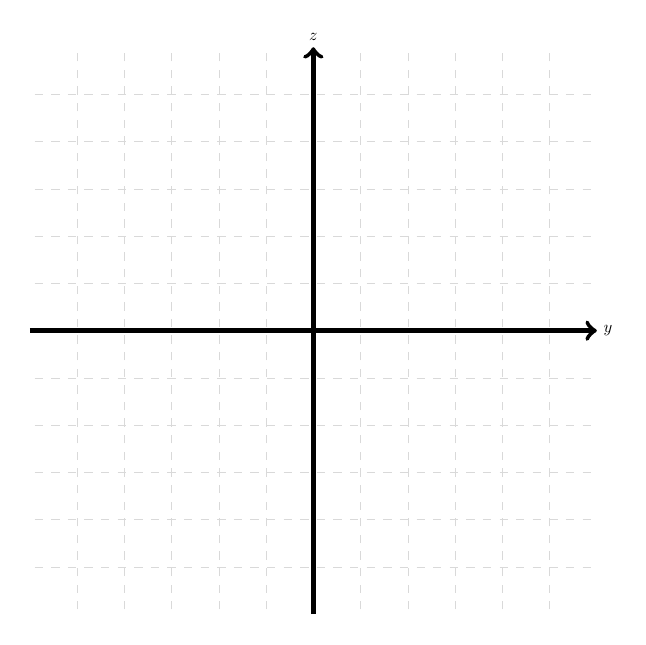
\begin{tikzpicture}[scale=0.6, transform shape]
\draw[help lines, color=gray!30, dashed] (-5.9,-5.9) grid (5.9,5.9);
\draw[->,ultra thick] (-6,0)--(6,0) node[right]{$y$};
\draw[->,ultra thick] (0,-6)--(0,6) node[above]{$z$};
\end{tikzpicture}
\end{center}
\vfill
\item[3] Sketch the traces of the form $y = k$, with $ k =0, 1 $ in the $xz$-plane where the $x$
axis is horizontal. Label your traces.
\begin{center}
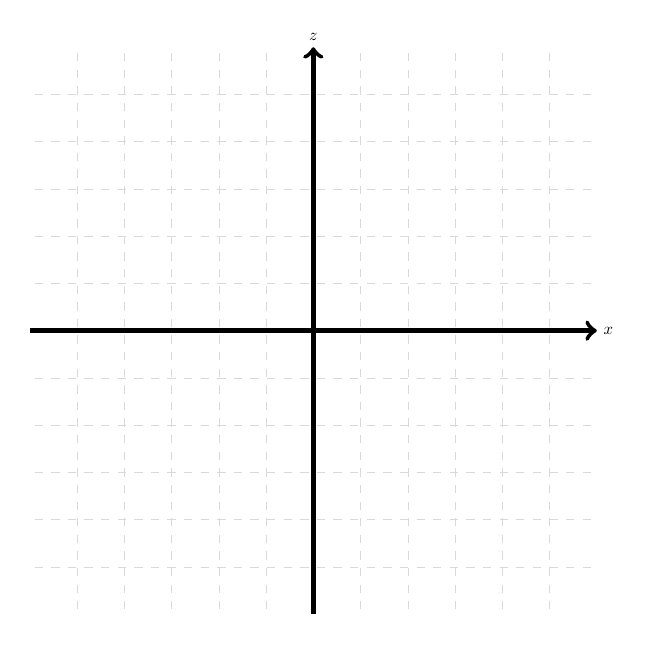
\begin{tikzpicture}[scale=0.6, transform shape]
\draw[help lines, color=gray!30, dashed] (-5.9,-5.9) grid (5.9,5.9);
\draw[->,ultra thick] (-6,0)--(6,0) node[right]{$x$};
\draw[->,ultra thick] (0,-6)--(0,6) node[above]{$z$};
\end{tikzpicture}
\end{center}
\vfill
\end{itemize}
\newpage
\item[10] If the limit exists, compute it (making sure to justify your answer). If the limit does
not exist, justify why it doesn’t exist. If you use a theorem, state clearly which theorem you are
using. Make sure to use correct limit notation.
$$\displaystyle\lim_{(x,y) \to (0,0)} \dfrac{xy^2}{2x^2 + y^4}$$
\vfill
\newpage
\item[7] At what point(s) does the curve $\vec{r}(t) = \langle 4t^2+6t, 0, t \rangle$ intersect
the paraboloid $x = y^2+z^2$ ? Make sure to give the coordinate(s) of the point(s) in your final
answer.
%At what point(s) does the curve $\vec{r}(t) = \langle t, 0, 2t-t^2 \rangle$ intersect the
% paraboloid $z = x^2+y^2$ ? Make sure to give the coordinate(s) of the point(s) in your final
% answer.
% CASSIE: This problem is #39 in 13.1, and a randomized version of it is on the 13.1
% homework.
\newpage
\item Consider the curve given by $\vec{r}(t)=\langle t, t^2, 2t+t^3\rangle.$
\begin{itemize}
\item[4] Find a tangent vector to the curve at the point $(2,4,12).$
\vfill
\item[4] Write down an integral that represents the length of the curve, with $1 \le t \le 2.$ You do
NOT need to evaluate the integral.
\vfill
\item[4] Find an equation for the tangent line to the curve at the point $(2,4,12).$
\vfill
\item[4] Find an equation for the normal plane to the curve at the point $(2,4,12).$ That is, find
an equation for the plane that is perpendicular to the tangent line to the curve at the given point.
\vfill
\vfill
\end{itemize}
\newpage
\item[7] Consider the surfaces $ z = \sqrt{x^2+y^2}$ and $ z = 2+x.$ Find a vector function
that represents the curve of intersection of the given surfaces.
\newpage
\item Consider the curve given by $\vec{r}(t)=\langle 3+2\sin(t),2t,2\cos(t)\rangle$
\begin{itemize}
\item[6] Find the unit tangent vector, $\vec{T}(t).$
\vfill
\item[6] Find the unit normal vector, $\vec{N}(t).$
\vfill
\item[4] Find the curvature, $\kappa(t).$
\vfill
\end{itemize}
\newpage
\item Consider the function $f(x,y) = \dfrac{\cos(y+x)}{ e^{x^2 -y}\sqrt{y^3-x}}.$
\begin{itemize}
\item[4] Find the domain of the function.
\vfill
\item[4] Sketch the domain of the function. Shade the region(s) that are part of the domain. Use
dotted lines when sketching a curve that is NOT in the domain, and solid lines when sketching
curves that are.
\vfill
\end{itemize}
\newpage
\item[8] An object's acceleration is given by
$$\vec{a}(t) = \langle \sin(\pi t), e^{-t}, 2t +3 \rangle.$$
Its initial velocity is $\vec{v}(0) = \langle 1,0,2 \rangle.$ Find a vector equation $\vec{v}(t)$ for
the velocity of the object at time $t.$
%\item[6] Find a vector equation $\vec{r}(t)$ for the position of the object at time $t.$
\newpage
\end{enumerate}
\end{document}